% !TEX root = main.tex
\subsection{Hahn echo}
\label{sec:Hahnecho}
Another relaxation measurement considers the time $T_2$, also referred to as the transversal relaxation time.
In order to understand that, we first have to explain the \textsc{Hahn} echo and the principle of multiple echo sequences.\newline
The principle of the \textsc{Hahn} echo is that an \SI{90}{\degree} pulse is applied and after a certain time $\tau$ a \SI{180}{\degree} pulse.
The reason behind this method is, that after the \SI{90}{\degree} pulse was applied the spins are oriented in the transversal plane and start to precess around the earths magnetic field vector (z-axis).
Due to spin-spin interaction (inhomogeneous magnetic field accrues) the spins also interact with each other and therefore some spins have a higher larmor frequency and some have a lower one.
If an \SI{180}{\degree} pulse is applied after a certain time the spins will flip in the transversal plane and the slow precessing spins will be located before the fast precessing spins again and when the fast precessing  overtake the slow ones the B$_1$ coil will detect a signal again.
The reason why the B$_1$ coil does not detect a signal while the slow and fast precessing spins are at different positions is that they erase each other, considering them as a superposition.
If the spin-spin interaction is too weak then it also helps to de-shim the system along the x-direction.
This also makes the homogeneous magnetic field inhomogeneous and thus the spins will get different larmor frequencies according to their position.\newline
Figure \ref{fig:Echobeispeilsignal} exemplary shows the \textsc{Hahn} echo for a shimming value of \SI{4.95}{\milli \ampere} along the x-axis (original value \SI{10.11}{\milli \ampere}).
It is also possible to change the time between the \SI{90}{\degree} and \SI{180}{\degree} pulse.
This would shift the peak to higher values in the timescale and due to loss effects, the amplitude would shrink a little bit.
\begin{figure}[H]
    \centering
    % GNUPLOT: LaTeX picture with Postscript
\begingroup
  % Encoding inside the plot.  In the header of your document, this encoding
  % should to defined, e.g., by using
  % \usepackage[cp1252,<other encodings>]{inputenc}
  \inputencoding{cp1252}%
  \makeatletter
  \providecommand\color[2][]{%
    \GenericError{(gnuplot) \space\space\space\@spaces}{%
      Package color not loaded in conjunction with
      terminal option `colourtext'%
    }{See the gnuplot documentation for explanation.%
    }{Either use 'blacktext' in gnuplot or load the package
      color.sty in LaTeX.}%
    \renewcommand\color[2][]{}%
  }%
  \providecommand\includegraphics[2][]{%
    \GenericError{(gnuplot) \space\space\space\@spaces}{%
      Package graphicx or graphics not loaded%
    }{See the gnuplot documentation for explanation.%
    }{The gnuplot epslatex terminal needs graphicx.sty or graphics.sty.}%
    \renewcommand\includegraphics[2][]{}%
  }%
  \providecommand\rotatebox[2]{#2}%
  \@ifundefined{ifGPcolor}{%
    \newif\ifGPcolor
    \GPcolorfalse
  }{}%
  \@ifundefined{ifGPblacktext}{%
    \newif\ifGPblacktext
    \GPblacktexttrue
  }{}%
  % define a \g@addto@macro without @ in the name:
  \let\gplgaddtomacro\g@addto@macro
  % define empty templates for all commands taking text:
  \gdef\gplbacktext{}%
  \gdef\gplfronttext{}%
  \makeatother
  \ifGPblacktext
    % no textcolor at all
    \def\colorrgb#1{}%
    \def\colorgray#1{}%
  \else
    % gray or color?
    \ifGPcolor
      \def\colorrgb#1{\color[rgb]{#1}}%
      \def\colorgray#1{\color[gray]{#1}}%
      \expandafter\def\csname LTw\endcsname{\color{white}}%
      \expandafter\def\csname LTb\endcsname{\color{black}}%
      \expandafter\def\csname LTa\endcsname{\color{black}}%
      \expandafter\def\csname LT0\endcsname{\color[rgb]{1,0,0}}%
      \expandafter\def\csname LT1\endcsname{\color[rgb]{0,1,0}}%
      \expandafter\def\csname LT2\endcsname{\color[rgb]{0,0,1}}%
      \expandafter\def\csname LT3\endcsname{\color[rgb]{1,0,1}}%
      \expandafter\def\csname LT4\endcsname{\color[rgb]{0,1,1}}%
      \expandafter\def\csname LT5\endcsname{\color[rgb]{1,1,0}}%
      \expandafter\def\csname LT6\endcsname{\color[rgb]{0,0,0}}%
      \expandafter\def\csname LT7\endcsname{\color[rgb]{1,0.3,0}}%
      \expandafter\def\csname LT8\endcsname{\color[rgb]{0.5,0.5,0.5}}%
    \else
      % gray
      \def\colorrgb#1{\color{black}}%
      \def\colorgray#1{\color[gray]{#1}}%
      \expandafter\def\csname LTw\endcsname{\color{white}}%
      \expandafter\def\csname LTb\endcsname{\color{black}}%
      \expandafter\def\csname LTa\endcsname{\color{black}}%
      \expandafter\def\csname LT0\endcsname{\color{black}}%
      \expandafter\def\csname LT1\endcsname{\color{black}}%
      \expandafter\def\csname LT2\endcsname{\color{black}}%
      \expandafter\def\csname LT3\endcsname{\color{black}}%
      \expandafter\def\csname LT4\endcsname{\color{black}}%
      \expandafter\def\csname LT5\endcsname{\color{black}}%
      \expandafter\def\csname LT6\endcsname{\color{black}}%
      \expandafter\def\csname LT7\endcsname{\color{black}}%
      \expandafter\def\csname LT8\endcsname{\color{black}}%
    \fi
  \fi
    \setlength{\unitlength}{0.0500bp}%
    \ifx\gptboxheight\undefined%
      \newlength{\gptboxheight}%
      \newlength{\gptboxwidth}%
      \newsavebox{\gptboxtext}%
    \fi%
    \setlength{\fboxrule}{0.5pt}%
    \setlength{\fboxsep}{1pt}%
\begin{picture}(7200.00,5040.00)%
    \gplgaddtomacro\gplbacktext{%
      \csname LTb\endcsname%%
      \put(814,704){\makebox(0,0)[r]{\strut{}$-60$}}%
      \put(814,1390){\makebox(0,0)[r]{\strut{}$-40$}}%
      \put(814,2076){\makebox(0,0)[r]{\strut{}$-20$}}%
      \put(814,2762){\makebox(0,0)[r]{\strut{}$0$}}%
      \put(814,3447){\makebox(0,0)[r]{\strut{}$20$}}%
      \put(814,4133){\makebox(0,0)[r]{\strut{}$40$}}%
      \put(814,4819){\makebox(0,0)[r]{\strut{}$60$}}%
      \put(946,484){\makebox(0,0){\strut{}$0$}}%
      \put(1727,484){\makebox(0,0){\strut{}$0.2$}}%
      \put(2508,484){\makebox(0,0){\strut{}$0.4$}}%
      \put(3289,484){\makebox(0,0){\strut{}$0.6$}}%
      \put(4070,484){\makebox(0,0){\strut{}$0.8$}}%
      \put(4851,484){\makebox(0,0){\strut{}$1$}}%
      \put(5632,484){\makebox(0,0){\strut{}$1.2$}}%
      \put(6413,484){\makebox(0,0){\strut{}$1.4$}}%
    }%
    \gplgaddtomacro\gplfronttext{%
      \csname LTb\endcsname%%
      \put(209,2761){\rotatebox{-270}{\makebox(0,0){\strut{}Amplitude in $\si{\mu \volt}$}}}%
      \put(3874,154){\makebox(0,0){\strut{}Time in $\si{\second}$}}%
      \csname LTb\endcsname%%
      \put(5816,4646){\makebox(0,0)[r]{\strut{}shimming value: $\SI{4.95}{\milli \ampere}$ along x-axis}}%
    }%
    \gplbacktext
    \put(0,0){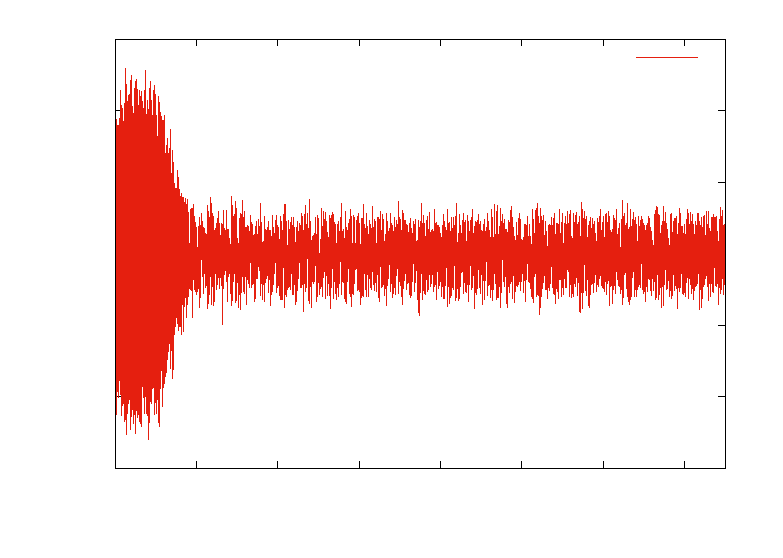
\includegraphics{plots/Echobeispeilsignal}}%
    \gplfronttext
  \end{picture}%
\endgroup

    \caption[Example measurement of a single \textsc{Hahn} echo for an echo time of \SI{0}{\milli \second}.]{Example measurement of a single \textsc{Hahn} echo for an echo time of \SI{0}{\milli \second}.
    The maximum of the echo is clearly visible.
    Due to relaxation after the maximum the detected signal at times after about \SI{0.2}{\second} is noise.}
    \label{fig:Echobeispeilsignal}
\end{figure}
It is also possible to fourier transform the signal from figure \ref{fig:Echobeispeilsignal}.
This is shown in figure \ref{fig:SpinEcho} for two different shimming values.
The amplitude of the spectrum with the shimming value of \SI{0}{\milli \ampere} along the x-axis is unambiguously smaller than the amplitude of the spectrum with shimming value of \SI{4.95}{\milli \ampere} along the x-axis.
This effect is a result of the more inhomogeneous magnetic field of the spectrum with the shimming value of \SI{0}{\milli \ampere} along the x-axis.
A more inhomogeneous magnetic field also has the consequence that the spins have more different larmor frequencies and thus the total intensity shrinks.
The area beneath the graph should be independent of the inhomogeneity because in total the magnetization has to be the same.
Only the distribution is different.
This effect is also clearly visible in figure \ref{fig:SpinEcho}.
This time it is not possible to find a good fitting function.
Therefore this discussion is more qualitative as mentioned before in chapter \ref{sec:OptimizationandCharacterisationofFIDinwatersample}.
The reason why there is no good fitting function is that there are a lot of randomly occurring peaks in the spectrum and the more peaks there are the more difficult it is to find a good fitting function.
Another thing that makes it rather hard is that the frequency steps are not quite small and thus there are few datapoints to make a good fit.
This also was a problem in chapter \ref{sec:OptimizationandCharacterisationofFIDinwatersample} as mentioned before.
\begin{figure}[H]
    \centering
    % GNUPLOT: LaTeX picture with Postscript
\begingroup
  % Encoding inside the plot.  In the header of your document, this encoding
  % should to defined, e.g., by using
  % \usepackage[cp1252,<other encodings>]{inputenc}
  \inputencoding{cp1252}%
  \makeatletter
  \providecommand\color[2][]{%
    \GenericError{(gnuplot) \space\space\space\@spaces}{%
      Package color not loaded in conjunction with
      terminal option `colourtext'%
    }{See the gnuplot documentation for explanation.%
    }{Either use 'blacktext' in gnuplot or load the package
      color.sty in LaTeX.}%
    \renewcommand\color[2][]{}%
  }%
  \providecommand\includegraphics[2][]{%
    \GenericError{(gnuplot) \space\space\space\@spaces}{%
      Package graphicx or graphics not loaded%
    }{See the gnuplot documentation for explanation.%
    }{The gnuplot epslatex terminal needs graphicx.sty or graphics.sty.}%
    \renewcommand\includegraphics[2][]{}%
  }%
  \providecommand\rotatebox[2]{#2}%
  \@ifundefined{ifGPcolor}{%
    \newif\ifGPcolor
    \GPcolorfalse
  }{}%
  \@ifundefined{ifGPblacktext}{%
    \newif\ifGPblacktext
    \GPblacktexttrue
  }{}%
  % define a \g@addto@macro without @ in the name:
  \let\gplgaddtomacro\g@addto@macro
  % define empty templates for all commands taking text:
  \gdef\gplbacktext{}%
  \gdef\gplfronttext{}%
  \makeatother
  \ifGPblacktext
    % no textcolor at all
    \def\colorrgb#1{}%
    \def\colorgray#1{}%
  \else
    % gray or color?
    \ifGPcolor
      \def\colorrgb#1{\color[rgb]{#1}}%
      \def\colorgray#1{\color[gray]{#1}}%
      \expandafter\def\csname LTw\endcsname{\color{white}}%
      \expandafter\def\csname LTb\endcsname{\color{black}}%
      \expandafter\def\csname LTa\endcsname{\color{black}}%
      \expandafter\def\csname LT0\endcsname{\color[rgb]{1,0,0}}%
      \expandafter\def\csname LT1\endcsname{\color[rgb]{0,1,0}}%
      \expandafter\def\csname LT2\endcsname{\color[rgb]{0,0,1}}%
      \expandafter\def\csname LT3\endcsname{\color[rgb]{1,0,1}}%
      \expandafter\def\csname LT4\endcsname{\color[rgb]{0,1,1}}%
      \expandafter\def\csname LT5\endcsname{\color[rgb]{1,1,0}}%
      \expandafter\def\csname LT6\endcsname{\color[rgb]{0,0,0}}%
      \expandafter\def\csname LT7\endcsname{\color[rgb]{1,0.3,0}}%
      \expandafter\def\csname LT8\endcsname{\color[rgb]{0.5,0.5,0.5}}%
    \else
      % gray
      \def\colorrgb#1{\color{black}}%
      \def\colorgray#1{\color[gray]{#1}}%
      \expandafter\def\csname LTw\endcsname{\color{white}}%
      \expandafter\def\csname LTb\endcsname{\color{black}}%
      \expandafter\def\csname LTa\endcsname{\color{black}}%
      \expandafter\def\csname LT0\endcsname{\color{black}}%
      \expandafter\def\csname LT1\endcsname{\color{black}}%
      \expandafter\def\csname LT2\endcsname{\color{black}}%
      \expandafter\def\csname LT3\endcsname{\color{black}}%
      \expandafter\def\csname LT4\endcsname{\color{black}}%
      \expandafter\def\csname LT5\endcsname{\color{black}}%
      \expandafter\def\csname LT6\endcsname{\color{black}}%
      \expandafter\def\csname LT7\endcsname{\color{black}}%
      \expandafter\def\csname LT8\endcsname{\color{black}}%
    \fi
  \fi
    \setlength{\unitlength}{0.0500bp}%
    \ifx\gptboxheight\undefined%
      \newlength{\gptboxheight}%
      \newlength{\gptboxwidth}%
      \newsavebox{\gptboxtext}%
    \fi%
    \setlength{\fboxrule}{0.5pt}%
    \setlength{\fboxsep}{1pt}%
\begin{picture}(7200.00,5040.00)%
    \gplgaddtomacro\gplbacktext{%
      \csname LTb\endcsname%%
      \put(682,704){\makebox(0,0)[r]{\strut{}$0$}}%
      \put(682,1253){\makebox(0,0)[r]{\strut{}$2$}}%
      \put(682,1801){\makebox(0,0)[r]{\strut{}$4$}}%
      \put(682,2350){\makebox(0,0)[r]{\strut{}$6$}}%
      \put(682,2899){\makebox(0,0)[r]{\strut{}$8$}}%
      \put(682,3447){\makebox(0,0)[r]{\strut{}$10$}}%
      \put(682,3996){\makebox(0,0)[r]{\strut{}$12$}}%
      \put(682,4545){\makebox(0,0)[r]{\strut{}$14$}}%
      \put(814,484){\makebox(0,0){\strut{}$1800$}}%
      \put(1563,484){\makebox(0,0){\strut{}$1810$}}%
      \put(2311,484){\makebox(0,0){\strut{}$1820$}}%
      \put(3060,484){\makebox(0,0){\strut{}$1830$}}%
      \put(3809,484){\makebox(0,0){\strut{}$1840$}}%
      \put(4557,484){\makebox(0,0){\strut{}$1850$}}%
      \put(5306,484){\makebox(0,0){\strut{}$1860$}}%
      \put(6054,484){\makebox(0,0){\strut{}$1870$}}%
      \put(6803,484){\makebox(0,0){\strut{}$1880$}}%
    }%
    \gplgaddtomacro\gplfronttext{%
      \csname LTb\endcsname%%
      \put(209,2761){\rotatebox{-270}{\makebox(0,0){\strut{}FID amplitude}}}%
      \put(3808,154){\makebox(0,0){\strut{}Frequency in $\si{}{Hz}$}}%
      \csname LTb\endcsname%%
      \put(5816,4646){\makebox(0,0)[r]{\strut{}shimmin value $x = \si{0}{}}}%
      \csname LTb\endcsname%%
      \put(5816,4426){\makebox(0,0)[r]{\strut{}shimmin value $x = \si{4.95}{}}}%
    }%
    \gplbacktext
    \put(0,0){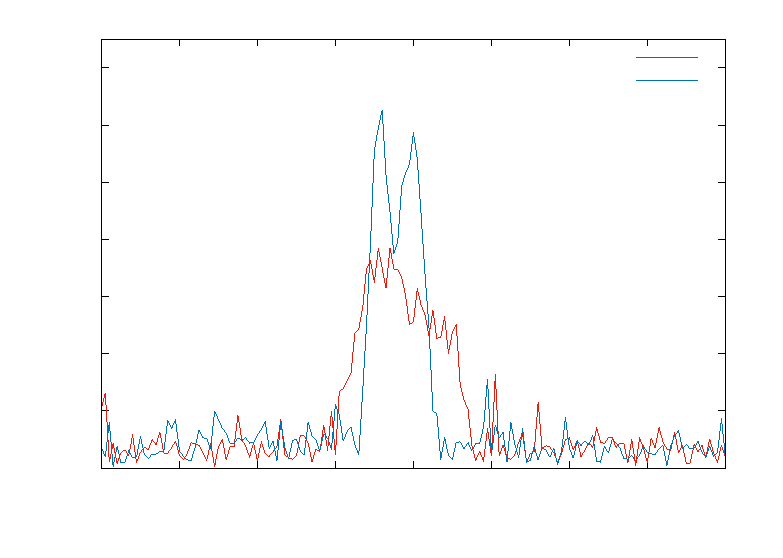
\includegraphics{plots/SpinEcho_4scans_ideal_Repetitiontime_0_shimming_150echo}}%
    \gplfronttext
  \end{picture}%
\endgroup

    \caption[Spectrum of a single \textsc{Hahn} echo applied by different shimming values.]{Spectrum of a single \textsc{Hahn} echo applied by different shimming values.
    Due to more de-shimming of the red curve, the amplitude is lower.
    Nevertheless the area under the spectrum is the same, due to the same magnetization.}
    \label{fig:SpinEcho}
\end{figure}
For the following chapter it is specifically important to know which relaxation time we observe.
Due to the inhomogeneous magnetic field there exist different relaxation times of the transversal relaxation time $T_2$.
The transversal relaxation time $T_2^*$ describes the relaxation in consideration of the inhomogeneous magentic field.
Therefore the formula has the following shape:
\begin{align}
    \frac{1}{T_2^*} = \frac{1}{T_2} + \gamma \Delta B_0 \ .
    \label{eq:T2_star}
\end{align}
In this equation $\gamma$ describes the gyromagnetic ratio of the probe and $\Delta B_0$ indicates the difference of the magnetic field to its equilibrium state.
Therefore we know that every time we de-shim the system $T_2^*$ is observed and not $T_2$.